\jxhj{%教学后记
	}
\skrq{%授课日期
	2017年12月26日 4-5节}
\ktmq{%课题名称
	 极坐标指令与实例}
\jxmb{%教学目标,每行前面要加 \item
	\item 掌握Fanuc上极坐标指令的使用;
	\item 掌握Siemens上极坐标指令的使用;
	\item 灵活使用极坐标指令进行编程;
	\item 掌握加工工艺的分析。
}
\jxzd{%教学重点,每行前面要加 \item
	\item Fanuc上极坐标指令的使用;
	\item Siemens上极坐标指令的使用。 }
\jxnd{%教学难点,每行前面要加 \item
	\item 使用极坐标指令进行编程。 }
\jjff{%教学方法
	通过讲述、举例、演示法来说明;}

\makeshouye %制作教案首页

%%%%教学内容
\subsection{组织教学}
\begin{enumerate}[\hspace{2em}1、]
	\item 集中学生注意力;
	\item 清查学生人数;
	\item 维持课堂纪律;
\end{enumerate}

\subsection{复习导入及主要内容}
\begin{enumerate}[1、]
\item 几种坐标系;
\item Fanuc 上局部坐标系;
\item Siemens 上局部坐标系;
\item 编程实例。
\end{enumerate}

\subsection{教学内容及过程}
\subsubsection{加工轮廓的处理}

\begin{figure}
	\centering
	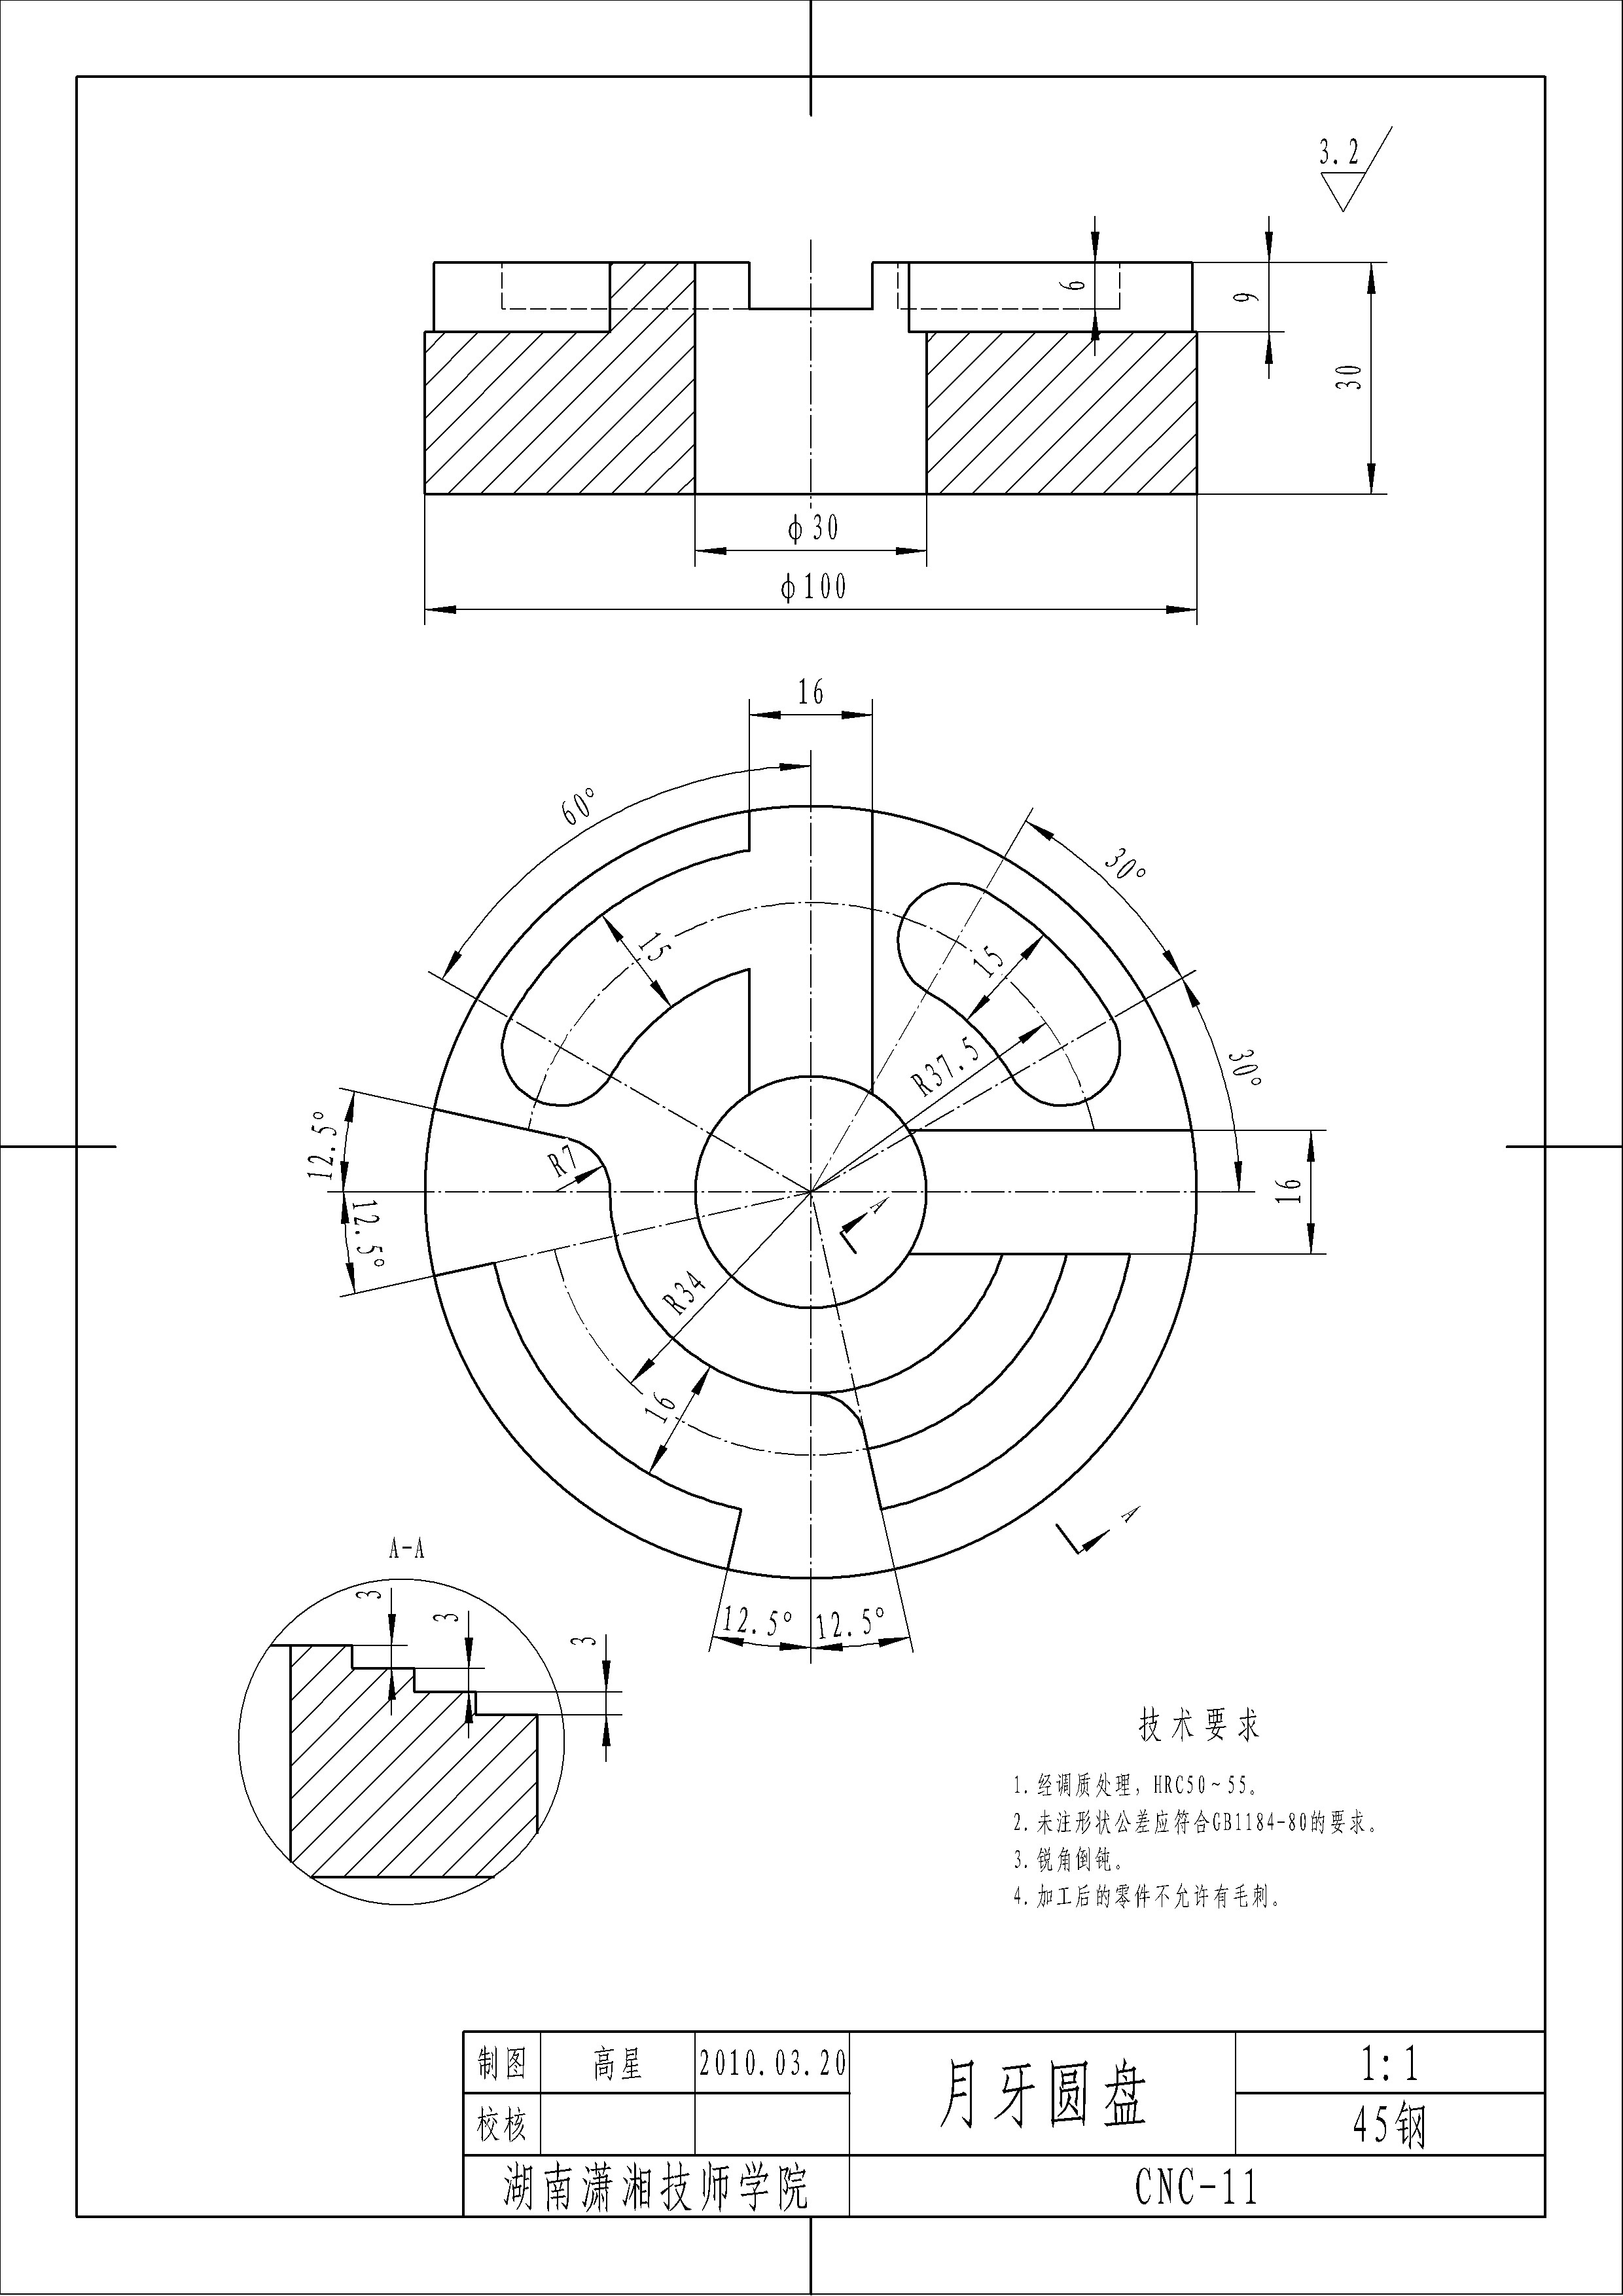
\includegraphics[width=0.9\linewidth,trim=50 150 50  50,clip]{data/image/30-1}
	\caption{加工轮廓的处理}
	\label{fig:30-1}
\end{figure}

1、加工轮廓的处理(改路径,延长)

把加工轮廓进行拆分

A、两个直槽:

标点的坐标,直角坐标(开放的)

B、小圆弧槽:

标点的坐标,使用极坐标

C、腰形槽:

标点的坐标,极坐标

D、扇形台阶

标点的坐标,极坐标

起点与终点不重合

编程时的处理

E、带翅膀的圆弧槽。

极坐标 与 直角坐标的互换。

X=P*cosA

Y=P*sinA

P=X2+Y2

A=aictanY/X

\subsubsection{极坐标}

1、Fanuc上的极坐标

指令格式: G\_\_ G~~ G16;启动极坐标指令(极坐标方式)
G~~ IP\_\_; 极坐标指令
:

G15;取消极坐标

说明:G\_\_ 极坐标指令的平面选择(G17、G18、G19)

G~~ G90指定工件坐标系的零点作为极坐标系原点,

G91指定当前位置作为极坐标系的原点。

IP\_\_\_ 指定极坐标系选择平面的轴地址及其值。

第1轴:极坐标半径

第2轴:极坐标角度 

用G90指定半径,极点设在工件坐标系原点。

如再用G90指定角度,角度是与X轴的夹角

如再用G91指定角度,角度是与当前位置的夹角

用G91指定半径,极点设在刀具当前位置。

如再用G90指定角度,角度是与X轴的夹角

如再用G91指定角度,角度是与当前位置的夹角。

限制:A、在极坐标方式中,对圆弧插补或螺旋线插补(G02,G03)用R 指定半径。

B、在极坐标方式中,不能用以下指令:

G4、G10、G52、G92、G53、G68、G51

C、在极坐标方式中不能倒角和倒圆

2、Siemens上的极坐标

1、极坐标,极点定义:G110,G111,G112 

A、在直角坐标系中定义极点:

G110/G111/G112 X\_\_ Y\_\_ Z\_\_ 

B、在极坐标系中定义极点:

G110/G111/G112 AP=\_\_\_ RP=\_\_\_

说明: 

G110:相对于刀具最近到达的点(刀具当前位置)定义极点

G111:相对于当前工件坐标系定义极点

G112:相对于上一个有效极点定义极点

2、在极坐标系中使用极坐标

A、G0 AP=\_\_\_ RP=\_\_\_\_

B、G1 AP=\_\_\_ RP=\_\_\_

C、G2 AP=\_\_\_ RP=\_\_\_

D、G3 AP=\_\_\_ RP=\_\_\_

说明:

AP=\_\_\_:极角,极点和目标点之间连线与角度参考方向之间的夹角(第
一次角度参考方向线中一条),取值范围±(0-360),当用绝对坐标编程时,角度为相对于加工平面的水平轴方向,当用相对坐标编程时,上一个被编程角度作为参考位置。极角一直保持到新的极角被定义或工件坐标系被改变。

RP=\_\_\_:极半径,极点和目标点之间的距离,极半径一保持到新的极半径被定义。

所有与极坐标有关的输入必须在单个程序段内编程。用极坐标所定义的位置都可以用G0 G1 G2 G3去移动,极坐系在由G17/G18/G19所定义的加工平面内都有效。如果没有极坐标在使用,有效的工件坐标系的原点有用,

\subsubsection{加工工序:(比较分析讲解)}

A、铣上表面

B、铣ф30通孔(也可钻、扩、镗)

C、铣直槽和圆弧

……

由学生自己分析。

\subsection{课堂小结}
\begin{enumerate}[1、]
\item 加工轮廓的处理;
\item 极坐标;
\item 编程实例。
\end{enumerate}

\vfill
\subsection{布置作业}
\begin{enumerate}[1、]
	\item 综合习题一。
\end{enumerate}
\vfill